\ifpdf
    \graphicspath{{figures/}{figures/comparisons}}
\else
    \graphicspath{{figures/}{figures/comparisons}}
\fi

% this file is called up by thesis.tex
% content in this file will be fed into the main document

\chapter{Fundamentals} % top level followed by section, subsection
This chapter explains the basic theory behind 3D reconstruction and Structure from Motion. All information referred to herein can be found in \cite{HartleyMultipleView}. It also includes a brief overview of sensors, which can be used to calculate global or relative orientation of the smartphone camera. It is also explained, why it is necessary to use accelerometer, gyroscope and magnetometer together by combing them into Sensor Fusion. 

% ----------------------- contents from here ------------------------
\section{3D reconstruction}
In general 3D reconstruction is the process of automatic creation of 3 dimensional objects models from images. There are many possibilities of performing 3D reconstruction, starting from two-view reconstruction, where only two images are used to multiple-view reconstruction, where image sequence is bigger than 2. Reconstruction can be performed either with a single hand-held camera from images sequence or simultaneously working and synchronised multiple cameras. It can be done either on spot in real time or later for instance in laboratory. As few as two pictures taken from different angles of a single object are sufficient to perform 3D model generation. In general reconstruction process consists of the following steps:
\setlist[2]{noitemsep} % sets the itemsep and parsep for all level two lists to 0
\setenumerate{noitemsep} % sets no itemsep for enumerate lists only
\begin{enumerate}
\item \textbf{Image Acquisition}, where images frames are acquired 
\item \textbf{Feature extraction and corresponding points matching}, where distinctive features are extracted from the images and compared
\item \textbf{Fundamental \& Essential Matrices computation}, where matrices meeting the requirements of basic epipolar geometry are calculated
\item \textbf{Camera parameters estimation}, where external and internal camera parameters, like translation and rotation are estimated
\item \textbf{Triangulation}, where camera projection matrices are composed and used in order to calculate 3D cloud points
\end{enumerate}
\subsection{Camera model}
To get reader acquainted with nomenclature used when reading about camera related operations following section was written. In general two coordinations system are related to camera model, which can be seen in Figure \ref{fig:camera_model}:
\begin{enumerate} 
\item The external coordinate system (denoted here with a subscript \textbf{W} for world) which is independent of placement and parameters of the camera.
\item The camera coordinate system (denoted by \textbf{C}, for camera).
\end{enumerate}
Relation between those two coordinate systems is expressed by translation matrix \textbf{T} and rotation matrix \textbf{R}. These two together are often referred as external camera parameters.
\begin{figure}[h!]
    \centering
    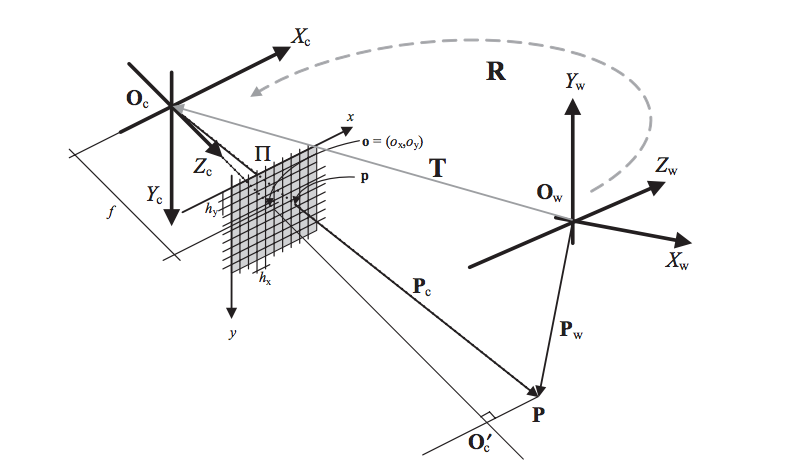
\includegraphics[width=0.8\textwidth]{camera_model}
    \caption{Model of the perspective camera with two coordinate systems: external W and
internal K. Image taken from \cite{Cyganek3dVision}.}
    \label{fig:camera_model}
\end{figure}
Internal camera parameters are expressed by the following matrix:
\begin{equation}
\begin{array}{lcl}
\textbf{K} & = &
\begin{bmatrix}
h_{x} & 0 & o_{x} \\ 
0 & h_{y} & o_{y} \\ 
0 & 0 & 1
\end{bmatrix}
\end{array}
\end{equation}
where $h_{x}$ and $h_{y}$ represent the focal length of the camera expressed in pixel dimensions in the x and y direction respectively. Similarly, point \textbf{o} = $(o_{x},o_{y})$ is the principal point of camera in pixel dimensions. These parameters need to be calculated only once for each camera model. Once they are known, camera can be described as calibrated. 
Calibration of cameras can be done with special reference boards of the known dimensions and characteristics. One of such boards (Figure \ref{fig:camera_model}) as well as sample code that allows to calibrate camera is available on OpenCV website \cite{website:cameraCalibration}.
\begin{figure}[h!]
    \centering
    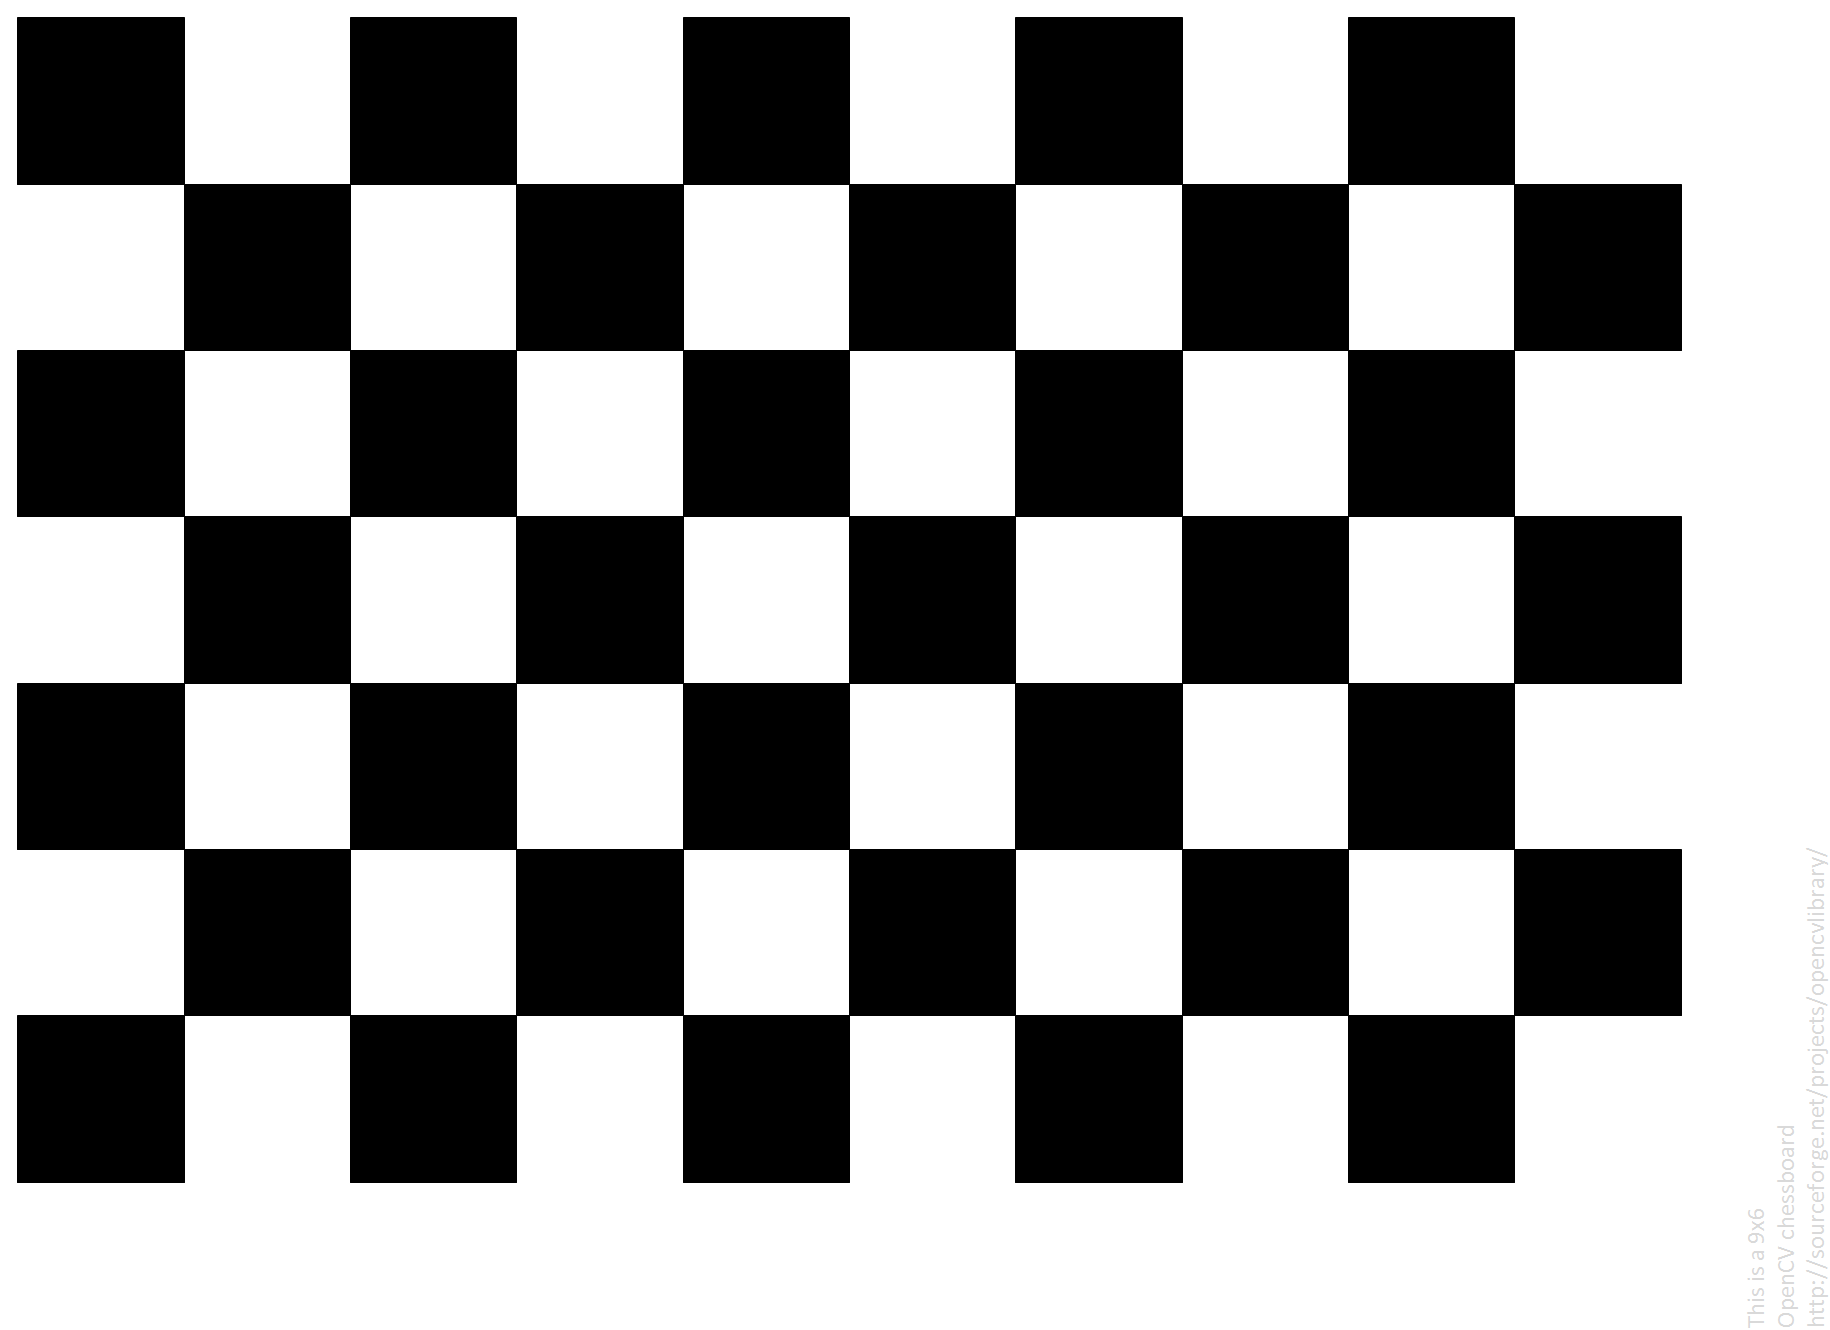
\includegraphics[width=0.8\textwidth]{opencv_camera_calib}
    \caption{OpenCV camera calibration board. Image taken from \cite{website:cameraCalibration}.}
    \label{fig:camera_model}
\end{figure}
Knowledge of external and internal camera parameters allows us to switch between camera and world coordinates system and is necessary for proper 3D model reconstruction.
\subsection{Feature extraction and corresponding points matching}
Usually, each image used in reconstruction has to be analysed in order for the distinctive features to be found. Afterwards all features in images are compared in order to find corresponding matches between them (Figure \ref{fig:correspondingMatches}).
\begin{figure}[h]
    \centering
    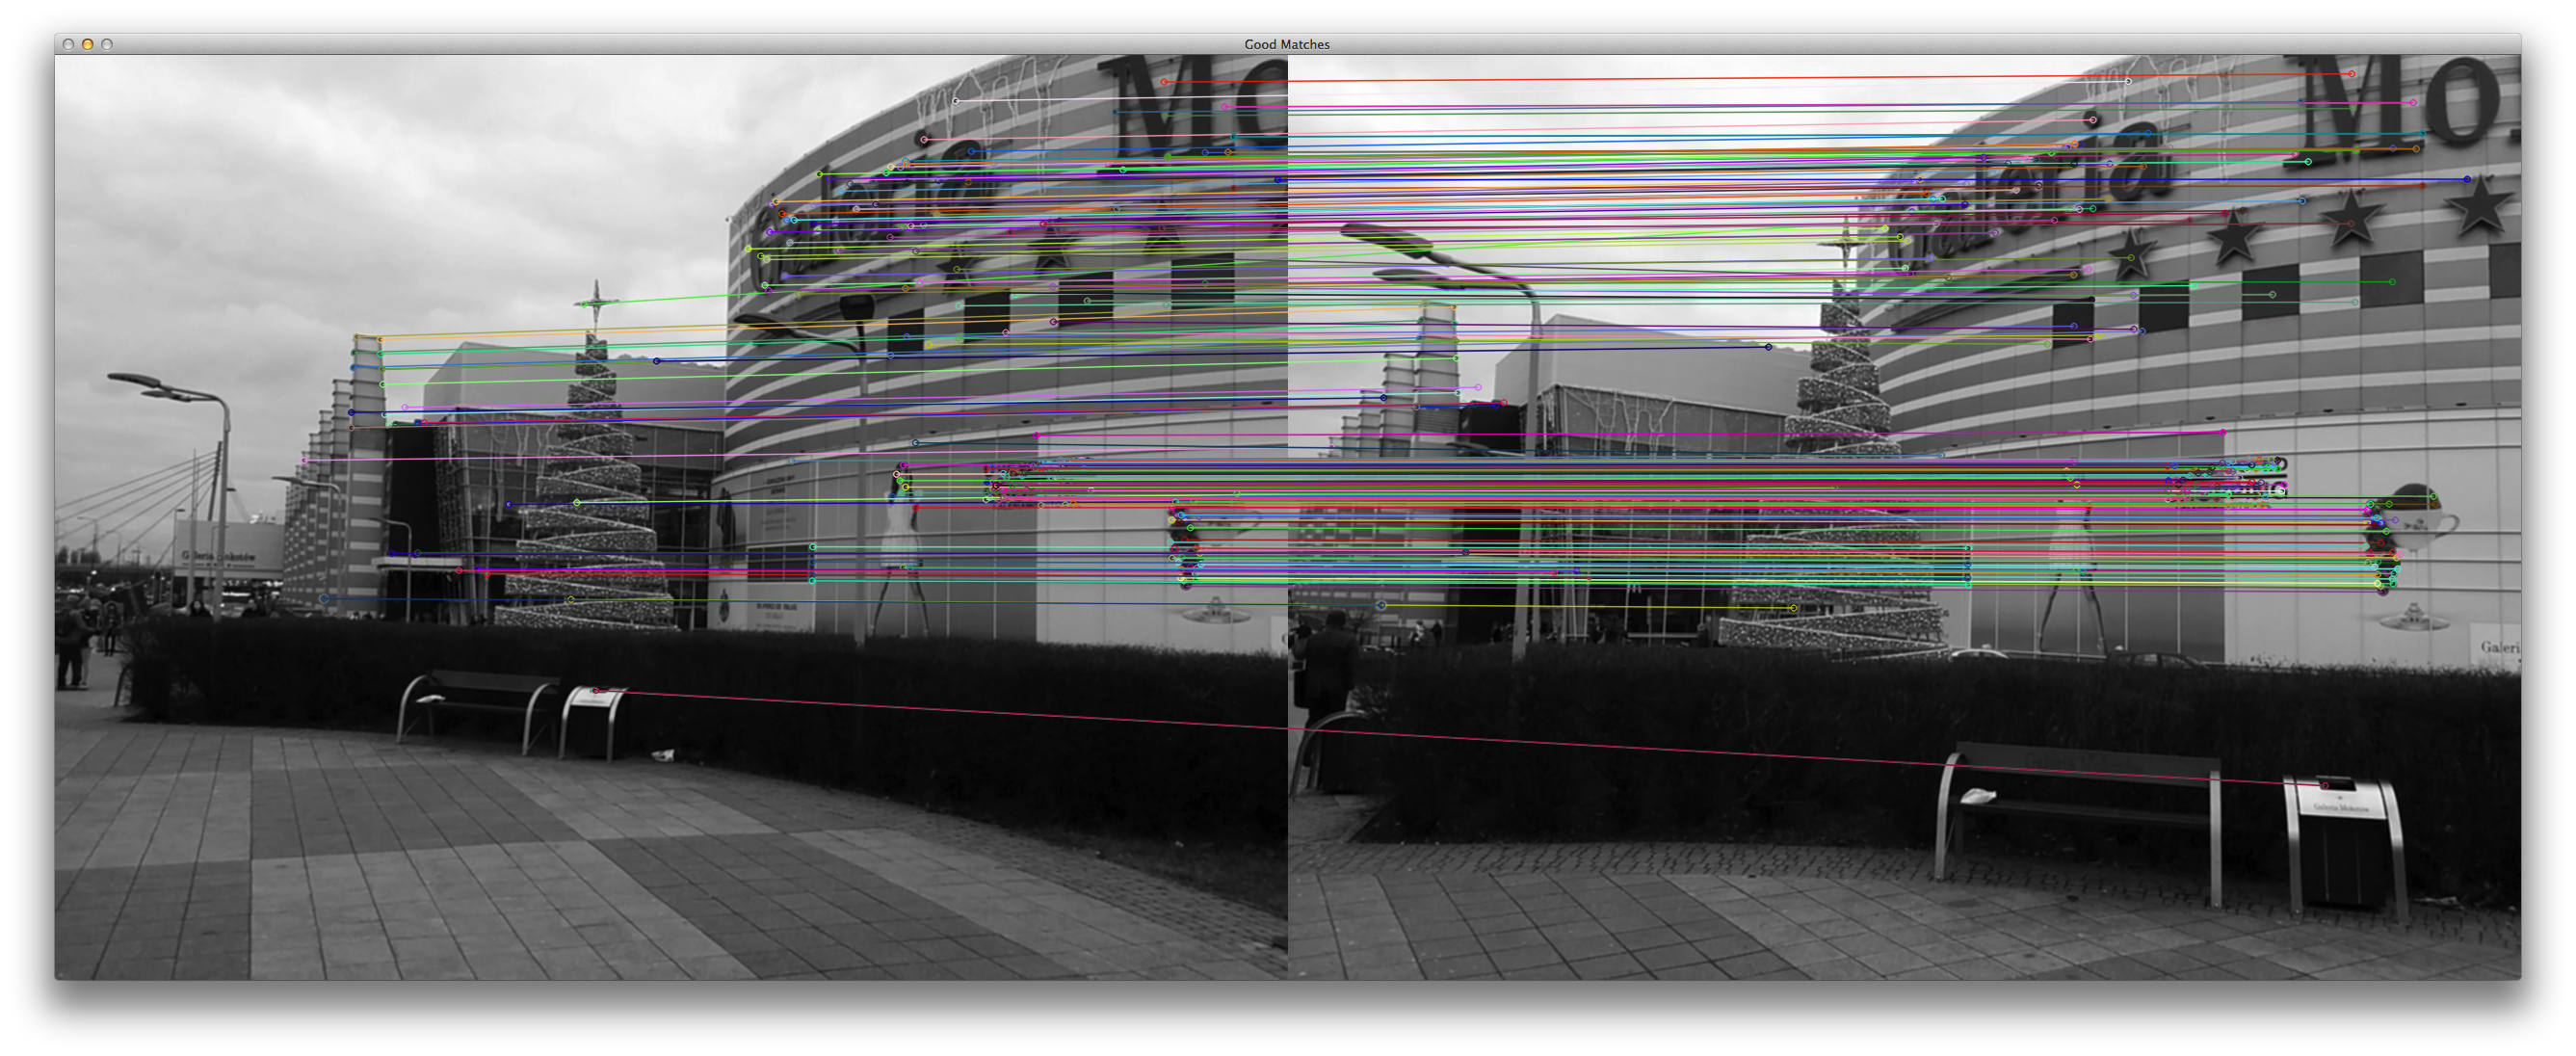
\includegraphics[width=0.8\textwidth]{correspondingMatching}
    \caption{Corresponding matches in ''Warsaw Gallery Dataset'' found for SIFT features and brute-force matcher using written by author desktop application}
    \label{fig:correspondingMatches}
\end{figure}
There are multiple features detectors and extractors available for use \cite{website:featureDetection}. Some of them are more suitable for edge detection, while others are best used for corner or blob based feature detection. One of the most popular and robust feature detection method is scale-invariant feature transform (SIFT) \cite{website:SIFT}. The use of these descriptors allows for detecting local features in images and describing them with special metrics, which are scale, rotation and translation invariant. Unfortunately even using such complex descriptors this process still is really hard and difficult. Algorithms that do these types of matching are usually O($n^2$) and therefore it takes a lot of time to find proper correspondences, especially when good object (image) resolution is needed. What is more even the most distinctive descriptors do not give global unique values and thus a lot of outliers can be produced during matching process (Figure \ref{fig:failMatching}). This is one of the first problems, which do not allow for perfectly accurate and error free 3D reconstruction.
\begin{figure}[ht!]
    \centering
    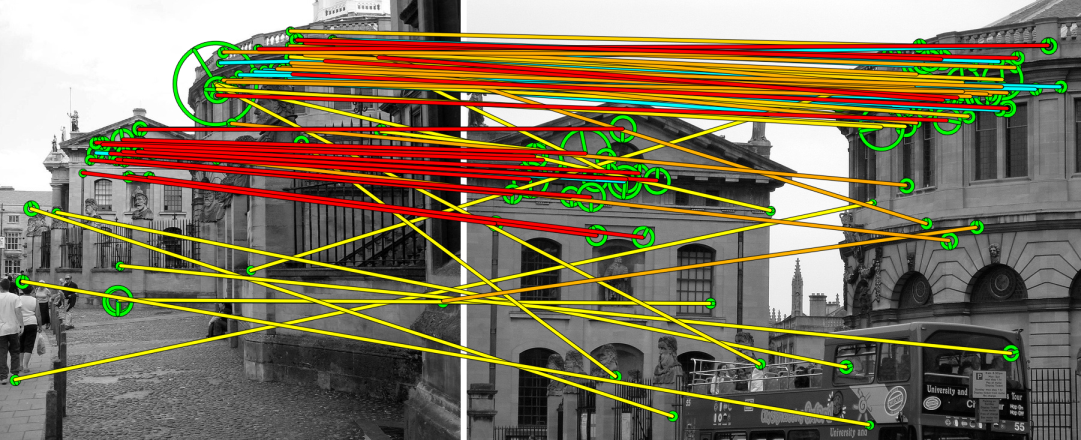
\includegraphics[width=0.8\textwidth]{failMatching}
    \caption[Outliers found during matching correspondences in two architecture pictures]{As shown in image example a lot of points in images can be improperly matched. This can influence further effectiveness of 3D reconstruction \cite{website:failMatching} }
    \label{fig:failMatching}
\end{figure}
\subsection{Epipolar geometry}
In Figure \ref{fig:epipolar_geometry} epipolar geometry schematic is shown. Baseline is the line connecting two cameras center points. Points in which baseline is crossing cameras image planes are called epipoles ($\textbf{e}_l$ and $\textbf{e}_r$). Lines that are going through epipoles and corresponding feature points $\textbf{p}_l$ and $\textbf{p}_r$ are called epipolar lines. Rays coming from cameras center points through corresponding feature points cross in position of 3D point \textbf{P} of photographed object.
\begin{figure}[!h]
    \centering
    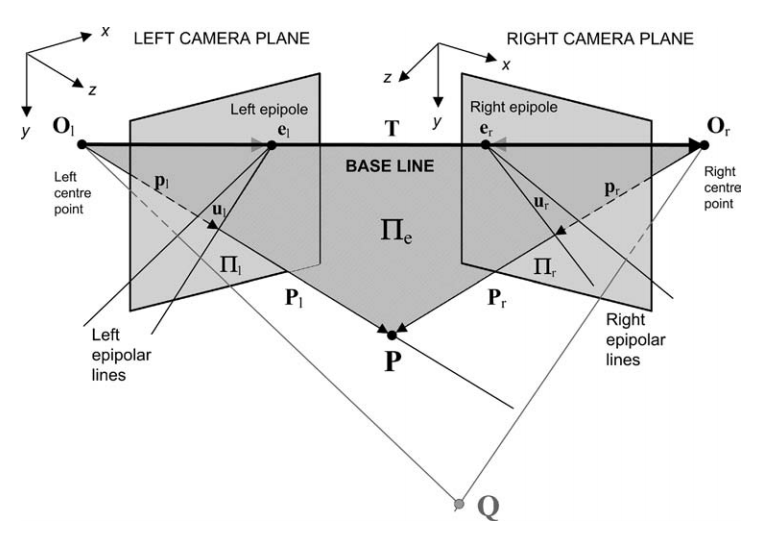
\includegraphics[width=0.8\textwidth]{epipolar_geometry}
    \caption{Epipolar geometry schematic. Picture from \cite{Cyganek3dVision}. }
    \label{fig:epipolar_geometry}
\end{figure}
Figure \ref{fig:EpipolarGeometry} shows different perspective on epipolar lines and example of their visualisation in image planes. These lines cross the exactly same points in both images and can be used for dense feature matching since matches need to be searched exclusively in the surroundings of these lines. However they can be calculated only if essential or fundmental matrix is determined.
\begin{figure}[!h]
    \centering
    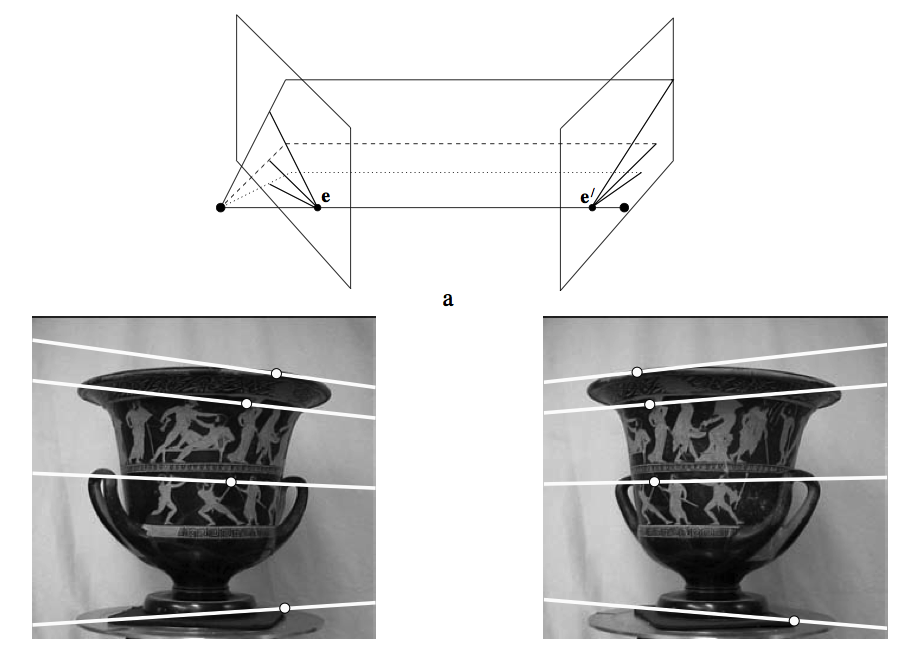
\includegraphics[width=0.8\textwidth]{EpipolarGeometry}
    \caption[Epipolar lines found in an image of a vase]{Epipolar lines found in an image of a vase \cite{HartleyMultipleView}. It is worth noting that all points that lay on corresponding epipolar lines and are visible in both images can be easily matched}
    \label{fig:EpipolarGeometry}
\end{figure} \\
\subsection{Fundamental \& Essential Matrix estimations}
Once proper feature matches are found in two images, it can be proven that there exists Fundamental matrix F for which the following equation is satisfied:
\begin{equation} \label{eq:fundamntalEquation}
\textbf{x}^{'T} \textbf{F} \textbf{x} = 0
\end{equation} 
where $x$ and ${x}^{'}$ are uncalibrated notions of points correspondence \cite{HartleyMultipleView}. It is known that solutions of this equation are highly sensitive to the occurrence of outliers. Usually, to make fundamental matrix estimations more accurate some outliers removing algorithms need to be used. One of the most robust approaches includes the use of of RANdom SAmple Consensus (RANSAC) \cite{website:ransac}.
\begin{figure}[h!]
    \centering
    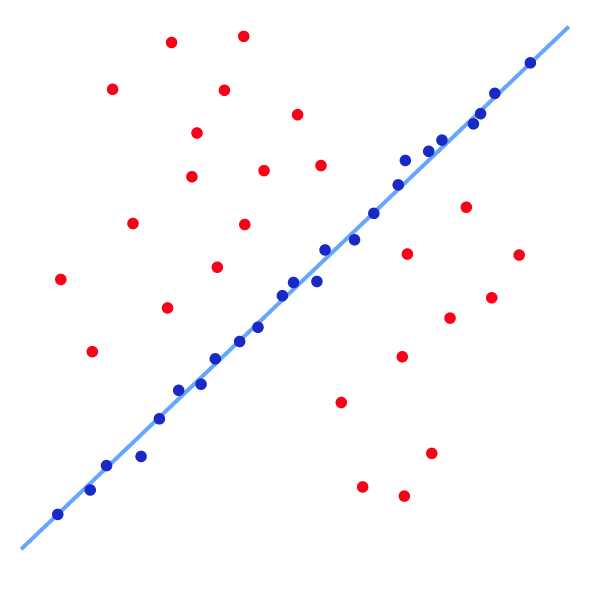
\includegraphics[width=0.8\textwidth]{RANSACFitting}
    \caption[RANSAC fitting for 2D image]{RANSAC fitting for 2D image\cite{website:ransac}. In this example all red points are some existing outliers. Blue line is decided by iterative process of fitting line to randomly chosen subset of all points. When enough percentage of all points lies in the neighbourhood of such fitted line(blue subset), process stops and unnecessary points (red points) can be removed for further processing.}
    \label{fig:RANSACFitting}
\end{figure}
Its basic idea relies on choosing a random subset from among all matches, solving a problem of reduced dataset and establishing how many points from the original set satisfy the equation. When enough inliers are found, points that do not satisfy the equation can be removed from further processing. The example 2 degree-of-freefom problem of sample fitting can be seen in Figure \ref{fig:RANSACFitting}. \\

When internal camera parameters K are known, the image points found can be calibrated and expressed in camera reference position system. Such calibrated points satisfy the following essential matrix E equation:
\begin{equation} \label{eq:essentialEquation}
\textbf{x}_{c}^{'T} \textbf{E} \textbf{x}_{c} = 0
\end{equation} 
which is very similar to a fundamental equation \ref{eq:fundamntalEquation}. This results in:
\begin{equation} \label{eq:essentialFundamentalRelation}
\textbf{E} = \textbf{K}^{T} \textbf{F} \textbf{K}
\end{equation} 
with \textbf{K} being matrix representing the internal camera parameters. 

The most known methods for Fundamental and Essential matrix calculations are:
\begin{enumerate}
\item{\textbf{8-point algorithm}} - 8 corresponding points pairs in image must be found and all of them are used in order to resolve 8DOF matrix problem and find fundamental matrix. More informations can be found in \cite{8Point}.
\item{\textbf{5-point algorithm}} - for calibrated cameras only 5 points pairs have to be used to resolve 5DOF matrix problem and find proper essential matrix. More informations can be found in \cite{iterative5point} or \cite{Batra5point}.
\end{enumerate}
Using Equation \ref{eq:essentialFundamentalRelation} one can go from Fundamental to Essential matrix and back. Next section will explain, how essential matrix is used in order to find relative translation and rotation between cameras.
\subsection{Essential matrix decomposition}
In section 9.6.1 of Multiple View Geometry in Computer Vision (\cite{HartleyMultipleView}) it is shown in detail, how essential matrix can be decomposed using Singular Value Decomposition (SVD) to relative camera rotation \textbf{R} and translation \textbf{t}. In general SVD relay on decomposition one matrix to three other matrices, which multiplied give the initially decomposed matrix and where middle one is diagonal matrix. \\ 
Unfortunately, there are four possible solutions for such decomposition of essential matrix and it is not always possible to identify the correct one, especially when there is lot of unsuccessfully removed outliers present in corresponding points set. Figure \ref{fig:fourAmbig} presents the four possible situations of decomposition \textbf{E} to \textbf{R} and \textbf{T}. 
\begin{figure}[h!]
    \centering
    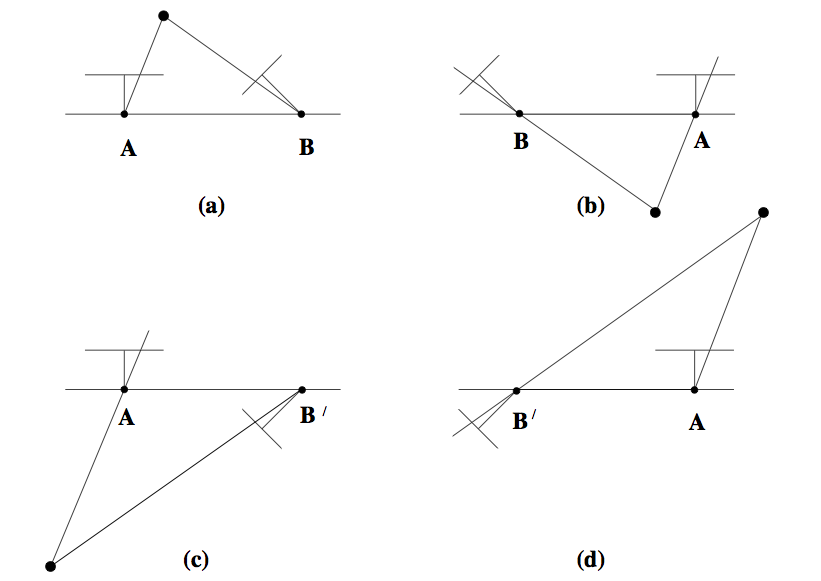
\includegraphics[width=0.8\textwidth]{fourAmbig}
    \caption[The four possible decompositions of \textbf{E}]{The four possible decompositions of \textbf{E}. Between the left and right sides there is a baseline reversal. Between the top and bottom rows camera B rotates 180$^{\circ}$ about baseline. Picture from page 260 of \cite{HartleyMultipleView}.}
    \label{fig:fourAmbig}
\end{figure}
\\
However it is worth noting, that only in (a) is the reconstructed point in front of both cameras. Usually to determine proper solution it is enough using each of corresponding feature point to calculate its 3D positions and perform simple test checking if it lies in front of both cameras image planes. It may seem simple task, but from computer perspective it's hard to determine proper decomposition, when not all of outliers were removed during feature matching phase. Often outliers pair will show itself in front of both cameras for not correct solution.
This is the place in reconstruction pipeline where additional sensor data can be used to determine proper solution. In fact Sensor Fusion data can limit E matrix decomposition only to two solutions - (a) and (b) cases from Figure \ref{fig:fourAmbig}). What is most important that even in presence of many outliers it will produce proper perceptible models (cases (a) and (b) are baseline reversal). This will be explained in detail, when discussing enhancements to 8 and 5 point algorithms.
\subsection{Points Triangulation} \label{sec:points_triangulation}
Once internal and external camera parameters are calculated, the triangulation can be performed in order to acquire an affine reconstruction model (Figure \ref{fig:3Dreconstruction}).
\begin{figure}[h]
    \centering
    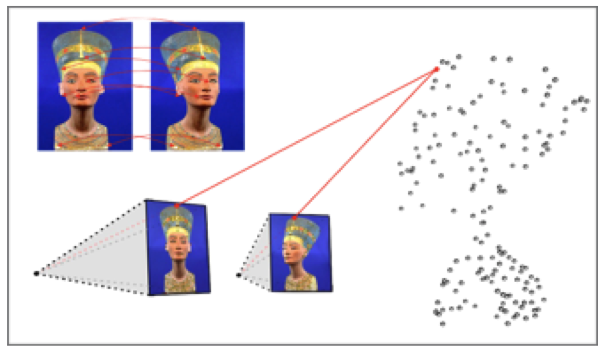
\includegraphics[width=0.8\textwidth]{3Dreconstruction}
    \caption[3D reconstruction from 2 images]{3D reconstruction from 2 images. Two rays crossing cameras centres and corresponding images points also cross in position of 3D point. [Slide from Photogrammetric Computer Vision from 2013/2014 winter semester at TU Berlin]}
    \label{fig:3Dreconstruction}
\end{figure}
Using \textbf{R} and \textbf{T} acquired from \textbf{E} decomposition and \textbf{K} from camera calibration, relation between 2D and 3D points can be expressed with following perspective projection matrices:
\begin{equation}
 \textbf{P}_{1} = \textbf{K} \begin{bmatrix}\textbf{I}\mid \textbf{0}\end{bmatrix} - \text{for first image,}
\end{equation}
\begin{equation}
 \textbf{P}_{2} = \textbf{K}  \begin{bmatrix}\textbf{R}\mid \textbf{t}\end{bmatrix} - \text{for second image,}
\end{equation}
where \textbf{I} is identity matrix, \textbf{0} is zero column vector, \textbf{R} is matrix representing relative rotation between cameras and \textbf{t} is relative translation vector between cameras. And now respectively:
\begin{equation}
 \textbf{x} = \textbf{P}_{1} \textbf{X} - \text{for first image,}
\end{equation}
\begin{equation}
 \textbf{x}^{'} = \textbf{P}_{2} \textbf{X} - \text{for second image,}
\end{equation}
where \textbf{X} is 3D position of point in space.
\\
Basically having relative cameras positions fully established (known internal parameters, rotation and translation) all rays connecting camera centres and corresponding image pairs will cross in place of their 3D location. Thus, it is worth noting here that resolution and density of 3D models rely on picture resolution and number of matching correspondences found. 
The only element that cannot be determined in such a case is the scale, because only relative positions between cameras can be established. This process is described in more details in Chapter 10 of Hartley's book\cite{HartleyMultipleView}.
\section{Structure from Motion}
The term ''Structure from Motion (SfM)'' refers to the reconstruction performed from the consecutive sequences of a moving camera. It is a popular research topic and the two main approaches, namely the Pose Estimation and Homography Estimation, can be used for the purposes of reconstructing a 3D model of an object visible throughout images sequence.
Lecture of this section give solid ground for understanding what Chapter\ref{chap:structure_from_motion} is about.
\subsection{3D Pose Estimation}
Assuming that some of the 3D cloud points are already known, the matches between 2D features in a new image and 3D point cloud positions can be established. Such 3D-2D matches can be used to estimate the camera position. This allows for reconstructing new 3D points and merging them smoothly into a functional model. Unfortunately,  this process is also highly sensitive to the occurrence of outliers, therefore adequate measures have to be undertaken to reduce their influence. One of the main advantages of this method is its speed. On the other hand, its effectiveness relies strongly on the initially existing 3D cloud quality. 
\subsection{Structure Adjustment}
Special refinement methods can be used to compensate for an error of mismatched points propagating through images. They include. among others, Bundle Adjustment (BA). The algorithm, using the information concerning the corresponding matches between multiple sets of images, iteratively modifies either both the camera external parameters and 3D points positions or one of them\cite{website:bundle-adjustment}. The main disadvantage of the method is its execution time. It is too time-consuming to be used in real-time applications. The basic idea of BA is expressed in Figure \ref{fig:BundleAdjustment}.
\begin{figure}[h]
    \centering
    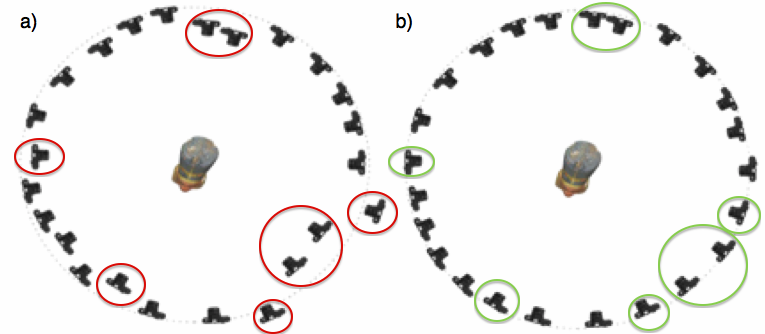
\includegraphics[width=0.8\textwidth]{BundleAdjustment}
    \caption[Bundle Adjustment process overview]{Bundle Adjustment process overview. Initially pictures around Pharaoh head from exactly the same distance on the circle. Due to presence of outliers, some of the estimated cameras were improperly estimated and  it could look like they were taken from different distances a). However after Bundle Adjustment process whole setup estimation was corrected to case b). Red circles indicates cameras, which positions were corrected in the process to the green ones. [Slide from Photogrammetric Computer Vision 2013/2014 winter semester at TU Berlin]}
    \label{fig:BundleAdjustment}
\end{figure}
Theoretically usage of Sensor Fusion initial rotation and translation estimation should produce close to actual values and thus result in better convergence speed during BA.
\section[Mobile Sensors overview]{Mobile Sensors overview\cite{website:androidSensorOverview}}
There are many sensors available in the nowadays smartphones, such as accelerometer, gyroscope, magnetometer, barometer, GPS, etc. All of them have their advantages and disadvantages, and thus the errors of some might be compensated with the strengths of the others in order to, for example, accurately compute camera rotation angles. Very good overview of sensors accuracy on example of Android can be found in Google Tech Talk called: "Sensor Fusion on Android Devices: A Revolution in Motion Processing" \cite{website:androidSensorFusion}.
\subsection[Accelerometer]{Accelerometer\cite{website:accelerometer}}
An accelerometer is a device that measures acceleration along 3 axes of the device. Generally, an accelerometer allows for measuring total acceleration by sensing what force is applied to its micro strings. An accelerometer, which lies still on a flat surface parallel to the Earth's surface will indicate approximately the value of earth's gravity acceleration (1G) - around 9.8 $\frac{m}{{s}^{2}}$. This gravitation vector can be used to calculate the relative camera rotation, but it is difficult to define to which direction the gravity vector points when the device is moving in not a linear manner and acceleration readings are the sum of gravity and movement acceleration. The gravity vector can be obtained from the accelerometer data, when the device is still and later tracked during unexpected movements with the usage of gyroscope sensor data. 
In case of Android accelerometers acceleration is returned in $\frac{m}{{s}^{2}}$.
\subsection[Gyroscope]{Gyroscope\cite{website:gyroscope}}
A gyroscope is a device for measuring or maintaining orientation, based on the principles of conservation of angular momentum. A standard gyroscope consists of a spinning wheel mounted on two gimbal rings, which allows it to rotate in all three axes. The spinning wheel will resist changes in orientation, due to an effect of the conservation of angular momentum. A conventional gyroscope measures orientation, in contrast to MEMS (Micro Electro-Mechanical System) types, which measure angular rate, and are therefore called rate-gyros. MEMS gyroscopes contain vibrating elements to measure the Coriolis effect. In the end the angular velocity can be calculated in each axis. It is important to note that whereas the accelerometer and the magnetometer measure acceleration and angle relative to the Earth, gyroscope measures angular velocity relative to the body.
In case of Android rate of rotation is returned in $\frac{rad}{s}$.
\subsection[Sensor Fusion]{Sensor Fusion\cite{website:sensorFustion}}
Sensor fusion is the process of combining sensory data derived from disparate sources in a way that the resulting information is to some extent more valuable than it would be possible should these sources be used individually. The term ''more valuable'' in this case may mean ''more accurate'', ''more complete'' or ''more dependable'', or refer to the result of an emerging view, such as stereoscopic vision (calculation of depth information by combining two-dimensional images from two cameras at slightly different viewpoints). 
In Android API available Sensor Fusion is made by combining accelerometer and gyroscope data. It allows on tracking gravity vector, which can be obtained when the device is not moving through rapid movements thanks to gyroscopic reading. The gravity vector can be decomposed in order to estimate the camera's rotation angles. In Figure \ref{fig:angles_from_gravity} reader can see overview of how gravity vector can be used to calculate rotation angles of the device. 
\begin{figure}[h!]
    \centering
    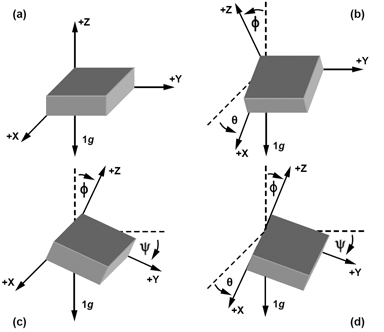
\includegraphics[width=0.8\textwidth]{angles_from_gravity}
    \caption[Getting rotation angles from gravity vector]{Getting rotation angles from gravity vector. In situation a) when device is not moving it is possible to determine the reference gravity vector values along each device axis. Later for situation b) to d) it is possible to calculate angles between current and reference gravity vector values on the corresponding device axes. Image from \cite{website:gravity_orientation}}
    \label{fig:angles_from_gravity}
\end{figure}
Unfortunately as shown for instance in \cite{sensorFusionSmartphones} and \cite{website:extendedSensorFusion} the calculated rotation angles may be few degrees drifted even when using Sensor Fusion. 
\\
Subtracting gravity from the actual acceleration measurements allows for estimating linear acceleration (Figure \ref{fig:linear_acceleration}). 
\begin{figure}[h!]
    \centering
    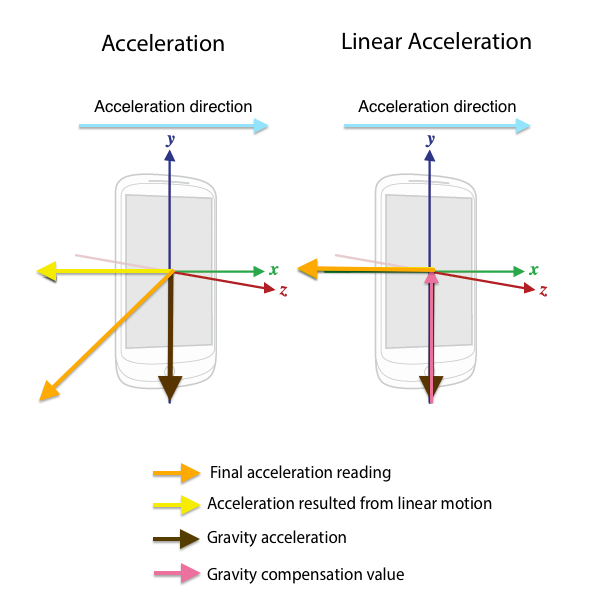
\includegraphics[width=0.8\textwidth]{linear_acceleration}
    \caption[Difference in readings of Android's acceleration and linear acceleration]{Difference in readings of Android's acceleration and linear acceleration. Having gravity vector pointing down (brown) and device accelerating in the right direction, acceleration vector (yellow) will show its minus influence on axis - x. For left situation when gravity vector is not known, final device acceleration readings will indicate orange value. However once gravity vector is known, its influence can be subtracted from acceleration reading, leaving pure device linear acceleration reading - right situation.}
    \label{fig:linear_acceleration}
\end{figure}
The use of linear acceleration makes it possible to measure the relative change of the device's translation. From fundamental physics distance traveled during acceleration movement moment is expressed by the following equation:
\begin{equation} \label{eq:trans_from_accel}
\textbf{s}_{\delta t} = \textbf{V}_{t} \cdot \delta t + \frac{\textbf{a} \cdot {\delta t}^{2}}{2},
\end{equation}
where $\textbf{V}_{t}$ represents current velocity of the device, $\delta t$ representing time difference, in which acceleration has happened and $\textbf{a}$ representing current linear acceleration vector. During acceleration velocity of the device changes according to following equation: 
\begin{equation}\label{eq:velo_accel}
\begin{array}{c}
\textbf{V}_{\delta t} = \textbf{a} \cdot \delta t \\
\textbf{V}_{t + \delta t} = \textbf{V}_{t} + \textbf{V}_{\delta t},
\end{array}
\end{equation}
However, as reader can see to get translation it is required to integrate acceleration over time twice, which can result in largely increasing the translation's estimation errors, when noisy data are available. 
As mentioned already in this section, \cite{website:androidSensorFusion} presents in particular how noisy mobile sensors prove to be in reality, especially when used during movement, thus translation estimation can be highly inaccurate.
Unfortunately there is no good official documentation, where Android linear acceleration reading error was calculated, but one of comprehensive study on Android Sensor Fusion and distance calculation using linear acceleration can be found in \cite{indoorPosition}. Also Chapter \ref{chap:recon_sensors} includes author's experiments on rotation and translation estimation using Sensor Fusion data.
% ---------------------------------------------------------------------------
% ----------------------- end of thesis sub-document ------------------------
% ---------------------------------------------------------------------------
